% Created by tikzDevice version 0.12.6 on 2026-03-25 11:27:52
% !TEX encoding = UTF-8 Unicode
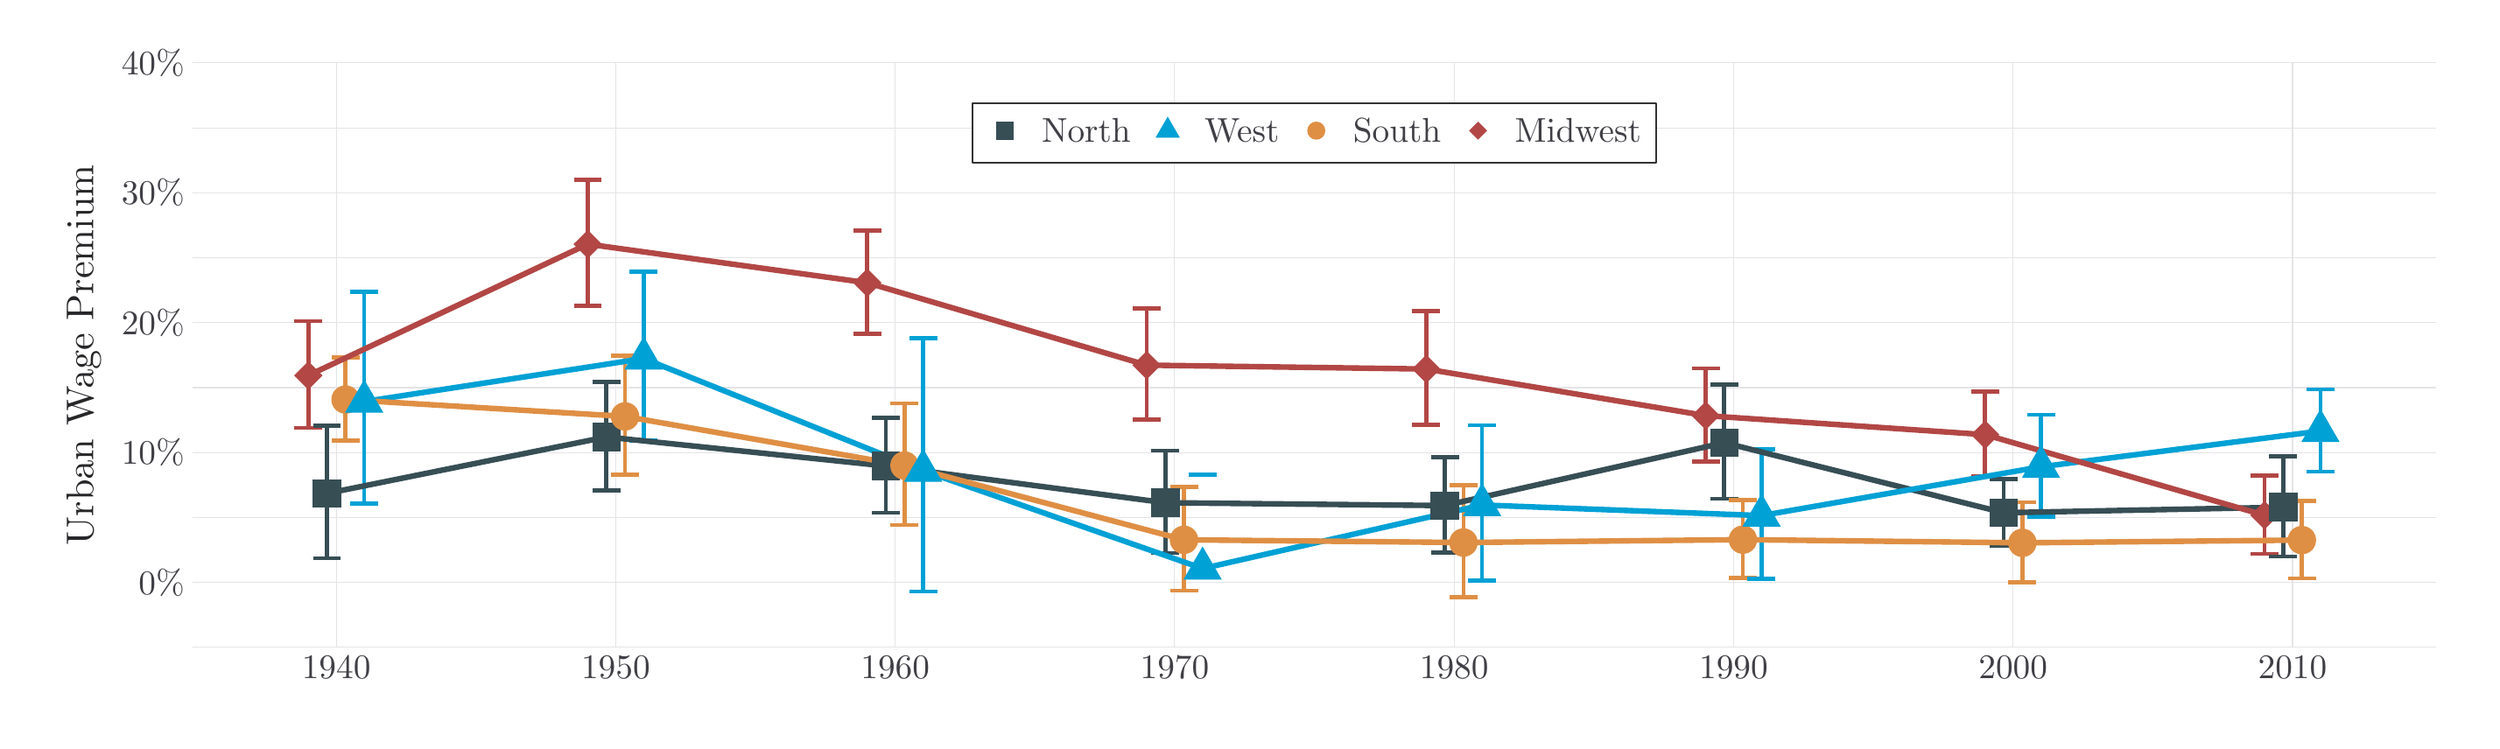
\begin{tikzpicture}[x=1pt,y=1pt]
\definecolor{fillColor}{RGB}{255,255,255}
\path[use as bounding box,fill=fillColor] (0,0) rectangle (1011.78,289.08);
\begin{scope}
\path[clip] (  0.00,  0.00) rectangle (1011.78,289.08);
\definecolor{drawColor}{RGB}{255,255,255}

\path[draw=drawColor,line width= 0.8pt,line join=round,line cap=round,fill=fillColor] (  0.00,  0.00) rectangle (1011.78,289.08);
\end{scope}
\begin{scope}
\path[clip] ( 69.39, 31.76) rectangle (995.78,273.08);
\definecolor{drawColor}{RGB}{255,255,255}
\definecolor{fillColor}{RGB}{255,255,255}

\path[draw=drawColor,line width= 0.8pt,line join=round,line cap=round,fill=fillColor] ( 69.39, 31.76) rectangle (995.78,273.08);
\definecolor{drawColor}{RGB}{228,228,231}

\path[draw=drawColor,line width= 0.4pt,line join=round] ( 69.39, 31.76) --
	(995.78, 31.76);

\path[draw=drawColor,line width= 0.4pt,line join=round] ( 69.39, 85.39) --
	(995.78, 85.39);

\path[draw=drawColor,line width= 0.4pt,line join=round] ( 69.39,139.01) --
	(995.78,139.01);

\path[draw=drawColor,line width= 0.4pt,line join=round] ( 69.39,192.64) --
	(995.78,192.64);

\path[draw=drawColor,line width= 0.4pt,line join=round] ( 69.39,246.27) --
	(995.78,246.27);

\path[draw=drawColor,line width= 0.4pt,line join=round] ( 69.39, 58.57) --
	(995.78, 58.57);

\path[draw=drawColor,line width= 0.4pt,line join=round] ( 69.39,112.20) --
	(995.78,112.20);

\path[draw=drawColor,line width= 0.4pt,line join=round] ( 69.39,165.83) --
	(995.78,165.83);

\path[draw=drawColor,line width= 0.4pt,line join=round] ( 69.39,219.45) --
	(995.78,219.45);

\path[draw=drawColor,line width= 0.4pt,line join=round] ( 69.39,273.08) --
	(995.78,273.08);

\path[draw=drawColor,line width= 0.4pt,line join=round] (128.81, 31.76) --
	(128.81,273.08);

\path[draw=drawColor,line width= 0.4pt,line join=round] (244.17, 31.76) --
	(244.17,273.08);

\path[draw=drawColor,line width= 0.4pt,line join=round] (359.54, 31.76) --
	(359.54,273.08);

\path[draw=drawColor,line width= 0.4pt,line join=round] (474.90, 31.76) --
	(474.90,273.08);

\path[draw=drawColor,line width= 0.4pt,line join=round] (590.27, 31.76) --
	(590.27,273.08);

\path[draw=drawColor,line width= 0.4pt,line join=round] (705.64, 31.76) --
	(705.64,273.08);

\path[draw=drawColor,line width= 0.4pt,line join=round] (821.00, 31.76) --
	(821.00,273.08);

\path[draw=drawColor,line width= 0.4pt,line join=round] (936.37, 31.76) --
	(936.37,273.08);
\definecolor{drawColor}{RGB}{178,71,69}

\path[draw=drawColor,line width= 1.7pt,line join=round] (111.50,166.46) --
	(123.04,166.46);

\path[draw=drawColor,line width= 1.7pt,line join=round] (117.27,166.46) --
	(117.27,122.38);

\path[draw=drawColor,line width= 1.7pt,line join=round] (111.50,122.38) --
	(123.04,122.38);
\definecolor{drawColor}{RGB}{55,78,85}

\path[draw=drawColor,line width= 1.7pt,line join=round] (119.19,123.40) --
	(130.73,123.40);

\path[draw=drawColor,line width= 1.7pt,line join=round] (124.96,123.40) --
	(124.96, 68.56);

\path[draw=drawColor,line width= 1.7pt,line join=round] (119.19, 68.56) --
	(130.73, 68.56);
\definecolor{drawColor}{RGB}{223,143,68}

\path[draw=drawColor,line width= 1.7pt,line join=round] (126.88,151.48) --
	(138.42,151.48);

\path[draw=drawColor,line width= 1.7pt,line join=round] (132.65,151.48) --
	(132.65,117.13);

\path[draw=drawColor,line width= 1.7pt,line join=round] (126.88,117.13) --
	(138.42,117.13);
\definecolor{drawColor}{RGB}{0,161,213}

\path[draw=drawColor,line width= 1.7pt,line join=round] (134.58,178.51) --
	(146.11,178.51);

\path[draw=drawColor,line width= 1.7pt,line join=round] (140.34,178.51) --
	(140.34, 91.10);

\path[draw=drawColor,line width= 1.7pt,line join=round] (134.58, 91.10) --
	(146.11, 91.10);
\definecolor{drawColor}{RGB}{178,71,69}

\path[draw=drawColor,line width= 1.7pt,line join=round] (226.87,224.82) --
	(238.40,224.82);

\path[draw=drawColor,line width= 1.7pt,line join=round] (232.64,224.82) --
	(232.64,172.68);

\path[draw=drawColor,line width= 1.7pt,line join=round] (226.87,172.68) --
	(238.40,172.68);
\definecolor{drawColor}{RGB}{55,78,85}

\path[draw=drawColor,line width= 1.7pt,line join=round] (234.56,141.47) --
	(246.10,141.47);

\path[draw=drawColor,line width= 1.7pt,line join=round] (240.33,141.47) --
	(240.33, 96.59);

\path[draw=drawColor,line width= 1.7pt,line join=round] (234.56, 96.59) --
	(246.10, 96.59);
\definecolor{drawColor}{RGB}{223,143,68}

\path[draw=drawColor,line width= 1.7pt,line join=round] (242.25,152.21) --
	(253.79,152.21);

\path[draw=drawColor,line width= 1.7pt,line join=round] (248.02,152.21) --
	(248.02,103.01);

\path[draw=drawColor,line width= 1.7pt,line join=round] (242.25,103.01) --
	(253.79,103.01);
\definecolor{drawColor}{RGB}{0,161,213}

\path[draw=drawColor,line width= 1.7pt,line join=round] (249.94,186.83) --
	(261.48,186.83);

\path[draw=drawColor,line width= 1.7pt,line join=round] (255.71,186.83) --
	(255.71,117.14);

\path[draw=drawColor,line width= 1.7pt,line join=round] (249.94,117.14) --
	(261.48,117.14);
\definecolor{drawColor}{RGB}{178,71,69}

\path[draw=drawColor,line width= 1.7pt,line join=round] (342.23,203.98) --
	(353.77,203.98);

\path[draw=drawColor,line width= 1.7pt,line join=round] (348.00,203.98) --
	(348.00,161.33);

\path[draw=drawColor,line width= 1.7pt,line join=round] (342.23,161.33) --
	(353.77,161.33);
\definecolor{drawColor}{RGB}{55,78,85}

\path[draw=drawColor,line width= 1.7pt,line join=round] (349.92,126.66) --
	(361.46,126.66);

\path[draw=drawColor,line width= 1.7pt,line join=round] (355.69,126.66) --
	(355.69, 87.29);

\path[draw=drawColor,line width= 1.7pt,line join=round] (349.92, 87.29) --
	(361.46, 87.29);
\definecolor{drawColor}{RGB}{223,143,68}

\path[draw=drawColor,line width= 1.7pt,line join=round] (357.62,132.52) --
	(369.15,132.52);

\path[draw=drawColor,line width= 1.7pt,line join=round] (363.38,132.52) --
	(363.38, 82.22);

\path[draw=drawColor,line width= 1.7pt,line join=round] (357.62, 82.22) --
	(369.15, 82.22);
\definecolor{drawColor}{RGB}{0,161,213}

\path[draw=drawColor,line width= 1.7pt,line join=round] (365.31,159.29) --
	(376.84,159.29);

\path[draw=drawColor,line width= 1.7pt,line join=round] (371.07,159.29) --
	(371.07, 54.78);

\path[draw=drawColor,line width= 1.7pt,line join=round] (365.31, 54.78) --
	(376.84, 54.78);
\definecolor{drawColor}{RGB}{178,71,69}

\path[draw=drawColor,line width= 1.7pt,line join=round] (457.60,171.63) --
	(469.14,171.63);

\path[draw=drawColor,line width= 1.7pt,line join=round] (463.37,171.63) --
	(463.37,125.77);

\path[draw=drawColor,line width= 1.7pt,line join=round] (457.60,125.77) --
	(469.14,125.77);
\definecolor{drawColor}{RGB}{55,78,85}

\path[draw=drawColor,line width= 1.7pt,line join=round] (465.29,112.98) --
	(476.83,112.98);

\path[draw=drawColor,line width= 1.7pt,line join=round] (471.06,112.98) --
	(471.06, 70.74);

\path[draw=drawColor,line width= 1.7pt,line join=round] (465.29, 70.74) --
	(476.83, 70.74);
\definecolor{drawColor}{RGB}{223,143,68}

\path[draw=drawColor,line width= 1.7pt,line join=round] (472.98, 97.92) --
	(484.52, 97.92);

\path[draw=drawColor,line width= 1.7pt,line join=round] (478.75, 97.92) --
	(478.75, 55.21);

\path[draw=drawColor,line width= 1.7pt,line join=round] (472.98, 55.21) --
	(484.52, 55.21);
\definecolor{drawColor}{RGB}{0,161,213}

\path[draw=drawColor,line width= 1.7pt,line join=round] (480.67,103.11) --
	(492.21,103.11);
\definecolor{drawColor}{RGB}{178,71,69}

\path[draw=drawColor,line width= 1.7pt,line join=round] (572.96,170.62) --
	(584.50,170.62);

\path[draw=drawColor,line width= 1.7pt,line join=round] (578.73,170.62) --
	(578.73,123.62);

\path[draw=drawColor,line width= 1.7pt,line join=round] (572.96,123.62) --
	(584.50,123.62);
\definecolor{drawColor}{RGB}{55,78,85}

\path[draw=drawColor,line width= 1.7pt,line join=round] (580.66,110.25) --
	(592.19,110.25);

\path[draw=drawColor,line width= 1.7pt,line join=round] (586.42,110.25) --
	(586.42, 71.00);

\path[draw=drawColor,line width= 1.7pt,line join=round] (580.66, 71.00) --
	(592.19, 71.00);
\definecolor{drawColor}{RGB}{223,143,68}

\path[draw=drawColor,line width= 1.7pt,line join=round] (588.35, 98.61) --
	(599.88, 98.61);

\path[draw=drawColor,line width= 1.7pt,line join=round] (594.12, 98.61) --
	(594.12, 52.41);

\path[draw=drawColor,line width= 1.7pt,line join=round] (588.35, 52.41) --
	(599.88, 52.41);
\definecolor{drawColor}{RGB}{0,161,213}

\path[draw=drawColor,line width= 1.7pt,line join=round] (596.04,123.51) --
	(607.57,123.51);

\path[draw=drawColor,line width= 1.7pt,line join=round] (601.81,123.51) --
	(601.81, 59.35);

\path[draw=drawColor,line width= 1.7pt,line join=round] (596.04, 59.35) --
	(607.57, 59.35);
\definecolor{drawColor}{RGB}{178,71,69}

\path[draw=drawColor,line width= 1.7pt,line join=round] (688.33,146.96) --
	(699.87,146.96);

\path[draw=drawColor,line width= 1.7pt,line join=round] (694.10,146.96) --
	(694.10,108.51);

\path[draw=drawColor,line width= 1.7pt,line join=round] (688.33,108.51) --
	(699.87,108.51);
\definecolor{drawColor}{RGB}{55,78,85}

\path[draw=drawColor,line width= 1.7pt,line join=round] (696.02,140.37) --
	(707.56,140.37);

\path[draw=drawColor,line width= 1.7pt,line join=round] (701.79,140.37) --
	(701.79, 93.09);

\path[draw=drawColor,line width= 1.7pt,line join=round] (696.02, 93.09) --
	(707.56, 93.09);
\definecolor{drawColor}{RGB}{223,143,68}

\path[draw=drawColor,line width= 1.7pt,line join=round] (703.71, 92.54) --
	(715.25, 92.54);

\path[draw=drawColor,line width= 1.7pt,line join=round] (709.48, 92.54) --
	(709.48, 60.37);

\path[draw=drawColor,line width= 1.7pt,line join=round] (703.71, 60.37) --
	(715.25, 60.37);
\definecolor{drawColor}{RGB}{0,161,213}

\path[draw=drawColor,line width= 1.7pt,line join=round] (711.40,113.61) --
	(722.94,113.61);

\path[draw=drawColor,line width= 1.7pt,line join=round] (717.17,113.61) --
	(717.17, 59.97);

\path[draw=drawColor,line width= 1.7pt,line join=round] (711.40, 59.97) --
	(722.94, 59.97);
\definecolor{drawColor}{RGB}{178,71,69}

\path[draw=drawColor,line width= 1.7pt,line join=round] (803.70,137.50) --
	(815.23,137.50);

\path[draw=drawColor,line width= 1.7pt,line join=round] (809.46,137.50) --
	(809.46,102.20);

\path[draw=drawColor,line width= 1.7pt,line join=round] (803.70,102.20) --
	(815.23,102.20);
\definecolor{drawColor}{RGB}{55,78,85}

\path[draw=drawColor,line width= 1.7pt,line join=round] (811.39,101.27) --
	(822.92,101.27);

\path[draw=drawColor,line width= 1.7pt,line join=round] (817.16,101.27) --
	(817.16, 73.73);

\path[draw=drawColor,line width= 1.7pt,line join=round] (811.39, 73.73) --
	(822.92, 73.73);
\definecolor{drawColor}{RGB}{223,143,68}

\path[draw=drawColor,line width= 1.7pt,line join=round] (819.08, 91.64) --
	(830.61, 91.64);

\path[draw=drawColor,line width= 1.7pt,line join=round] (824.85, 91.64) --
	(824.85, 58.68);

\path[draw=drawColor,line width= 1.7pt,line join=round] (819.08, 58.68) --
	(830.61, 58.68);
\definecolor{drawColor}{RGB}{0,161,213}

\path[draw=drawColor,line width= 1.7pt,line join=round] (826.77,127.77) --
	(838.31,127.77);

\path[draw=drawColor,line width= 1.7pt,line join=round] (832.54,127.77) --
	(832.54, 85.61);

\path[draw=drawColor,line width= 1.7pt,line join=round] (826.77, 85.61) --
	(838.31, 85.61);
\definecolor{drawColor}{RGB}{178,71,69}

\path[draw=drawColor,line width= 1.7pt,line join=round] (919.06,102.67) --
	(930.60,102.67);

\path[draw=drawColor,line width= 1.7pt,line join=round] (924.83,102.67) --
	(924.83, 70.36);

\path[draw=drawColor,line width= 1.7pt,line join=round] (919.06, 70.36) --
	(930.60, 70.36);
\definecolor{drawColor}{RGB}{55,78,85}

\path[draw=drawColor,line width= 1.7pt,line join=round] (926.75,110.76) --
	(938.29,110.76);

\path[draw=drawColor,line width= 1.7pt,line join=round] (932.52,110.76) --
	(932.52, 69.22);

\path[draw=drawColor,line width= 1.7pt,line join=round] (926.75, 69.22) --
	(938.29, 69.22);
\definecolor{drawColor}{RGB}{223,143,68}

\path[draw=drawColor,line width= 1.7pt,line join=round] (934.44, 92.32) --
	(945.98, 92.32);

\path[draw=drawColor,line width= 1.7pt,line join=round] (940.21, 92.32) --
	(940.21, 60.20);

\path[draw=drawColor,line width= 1.7pt,line join=round] (934.44, 60.20) --
	(945.98, 60.20);
\definecolor{drawColor}{RGB}{0,161,213}

\path[draw=drawColor,line width= 1.7pt,line join=round] (942.13,138.30) --
	(953.67,138.30);

\path[draw=drawColor,line width= 1.7pt,line join=round] (947.90,138.30) --
	(947.90,104.35);

\path[draw=drawColor,line width= 1.7pt,line join=round] (942.13,104.35) --
	(953.67,104.35);
\definecolor{drawColor}{RGB}{55,78,85}

\path[draw=drawColor,line width= 2.3pt,line join=round] (124.96, 95.32) --
	(240.33,118.61) --
	(355.69,106.64) --
	(471.06, 91.46) --
	(586.42, 90.29) --
	(701.79,116.26) --
	(817.16, 87.33) --
	(932.52, 89.61);
\definecolor{drawColor}{RGB}{0,161,213}

\path[draw=drawColor,line width= 2.3pt,line join=round] (140.34,133.24) --
	(255.71,151.02) --
	(371.07,104.70) --
	(486.44, 64.29) --
	(601.81, 90.53) --
	(717.17, 86.15) --
	(832.54,106.31) --
	(947.90,121.08);
\definecolor{drawColor}{RGB}{223,143,68}

\path[draw=drawColor,line width= 2.3pt,line join=round] (132.65,134.07) --
	(248.02,127.11) --
	(363.38,106.83) --
	(478.75, 76.15) --
	(594.12, 75.03) --
	(709.48, 76.22) --
	(824.85, 74.91) --
	(940.21, 76.03);
\definecolor{drawColor}{RGB}{178,71,69}

\path[draw=drawColor,line width= 2.3pt,line join=round] (117.27,144.03) --
	(232.64,198.25) --
	(348.00,182.31) --
	(463.37,148.28) --
	(578.73,146.68) --
	(694.10,127.43) --
	(809.46,119.59) --
	(924.83, 86.28);
\definecolor{fillColor}{RGB}{178,71,69}

\path[fill=fillColor] (111.40,144.03) --
	(117.27,149.91) --
	(123.14,144.03) --
	(117.27,138.16) --
	cycle;
\definecolor{fillColor}{RGB}{55,78,85}

\path[fill=fillColor] (119.09, 89.45) --
	(130.83, 89.45) --
	(130.83,101.20) --
	(119.09,101.20) --
	cycle;
\definecolor{fillColor}{RGB}{223,143,68}

\path[fill=fillColor] (132.65,134.07) circle (  5.87);
\definecolor{fillColor}{RGB}{0,161,213}

\path[fill=fillColor] (140.34,142.37) --
	(148.25,128.68) --
	(132.43,128.68) --
	cycle;
\definecolor{fillColor}{RGB}{178,71,69}

\path[fill=fillColor] (226.76,198.25) --
	(232.64,204.12) --
	(238.51,198.25) --
	(232.64,192.38) --
	cycle;
\definecolor{fillColor}{RGB}{55,78,85}

\path[fill=fillColor] (234.45,112.74) --
	(246.20,112.74) --
	(246.20,124.48) --
	(234.45,124.48) --
	cycle;
\definecolor{fillColor}{RGB}{223,143,68}

\path[fill=fillColor] (248.02,127.11) circle (  5.87);
\definecolor{fillColor}{RGB}{0,161,213}

\path[fill=fillColor] (255.71,160.15) --
	(263.62,146.46) --
	(247.80,146.46) --
	cycle;
\definecolor{fillColor}{RGB}{178,71,69}

\path[fill=fillColor] (342.13,182.31) --
	(348.00,188.19) --
	(353.87,182.31) --
	(348.00,176.44) --
	cycle;
\definecolor{fillColor}{RGB}{55,78,85}

\path[fill=fillColor] (349.82,100.77) --
	(361.56,100.77) --
	(361.56,112.51) --
	(349.82,112.51) --
	cycle;
\definecolor{fillColor}{RGB}{223,143,68}

\path[fill=fillColor] (363.38,106.83) circle (  5.87);
\definecolor{fillColor}{RGB}{0,161,213}

\path[fill=fillColor] (371.07,113.83) --
	(378.98,100.13) --
	(363.17,100.13) --
	cycle;
\definecolor{fillColor}{RGB}{178,71,69}

\path[fill=fillColor] (457.50,148.28) --
	(463.37,154.15) --
	(469.24,148.28) --
	(463.37,142.41) --
	cycle;
\definecolor{fillColor}{RGB}{55,78,85}

\path[fill=fillColor] (465.19, 85.59) --
	(476.93, 85.59) --
	(476.93, 97.34) --
	(465.19, 97.34) --
	cycle;
\definecolor{fillColor}{RGB}{223,143,68}

\path[fill=fillColor] (478.75, 76.15) circle (  5.87);
\definecolor{fillColor}{RGB}{0,161,213}

\path[fill=fillColor] (486.44, 73.42) --
	(494.35, 59.72) --
	(478.53, 59.72) --
	cycle;
\definecolor{fillColor}{RGB}{178,71,69}

\path[fill=fillColor] (572.86,146.68) --
	(578.73,152.55) --
	(584.61,146.68) --
	(578.73,140.81) --
	cycle;
\definecolor{fillColor}{RGB}{55,78,85}

\path[fill=fillColor] (580.55, 84.41) --
	(592.30, 84.41) --
	(592.30, 96.16) --
	(580.55, 96.16) --
	cycle;
\definecolor{fillColor}{RGB}{223,143,68}

\path[fill=fillColor] (594.12, 75.03) circle (  5.87);
\definecolor{fillColor}{RGB}{0,161,213}

\path[fill=fillColor] (601.81, 99.66) --
	(609.71, 85.96) --
	(593.90, 85.96) --
	cycle;
\definecolor{fillColor}{RGB}{178,71,69}

\path[fill=fillColor] (688.23,127.43) --
	(694.10,133.30) --
	(699.97,127.43) --
	(694.10,121.56) --
	cycle;
\definecolor{fillColor}{RGB}{55,78,85}

\path[fill=fillColor] (695.92,110.39) --
	(707.66,110.39) --
	(707.66,122.13) --
	(695.92,122.13) --
	cycle;
\definecolor{fillColor}{RGB}{223,143,68}

\path[fill=fillColor] (709.48, 76.22) circle (  5.87);
\definecolor{fillColor}{RGB}{0,161,213}

\path[fill=fillColor] (717.17, 95.28) --
	(725.08, 81.59) --
	(709.26, 81.59) --
	cycle;
\definecolor{fillColor}{RGB}{178,71,69}

\path[fill=fillColor] (803.59,119.59) --
	(809.46,125.46) --
	(815.34,119.59) --
	(809.46,113.72) --
	cycle;
\definecolor{fillColor}{RGB}{55,78,85}

\path[fill=fillColor] (811.28, 81.46) --
	(823.03, 81.46) --
	(823.03, 93.21) --
	(811.28, 93.21) --
	cycle;
\definecolor{fillColor}{RGB}{223,143,68}

\path[fill=fillColor] (824.85, 74.91) circle (  5.87);
\definecolor{fillColor}{RGB}{0,161,213}

\path[fill=fillColor] (832.54,115.44) --
	(840.45,101.74) --
	(824.63,101.74) --
	cycle;
\definecolor{fillColor}{RGB}{178,71,69}

\path[fill=fillColor] (918.96, 86.28) --
	(924.83, 92.16) --
	(930.70, 86.28) --
	(924.83, 80.41) --
	cycle;
\definecolor{fillColor}{RGB}{55,78,85}

\path[fill=fillColor] (926.65, 83.74) --
	(938.39, 83.74) --
	(938.39, 95.48) --
	(926.65, 95.48) --
	cycle;
\definecolor{fillColor}{RGB}{223,143,68}

\path[fill=fillColor] (940.21, 76.03) circle (  5.87);
\definecolor{fillColor}{RGB}{0,161,213}

\path[fill=fillColor] (947.90,130.21) --
	(955.81,116.52) --
	(939.99,116.52) --
	cycle;
\end{scope}
\begin{scope}
\path[clip] (  0.00,  0.00) rectangle (1011.78,289.08);
\definecolor{drawColor}{RGB}{63,63,70}

\node[text=drawColor,anchor=base east,inner sep=0pt, outer sep=0pt, scale=  1.42] at ( 66.19, 53.67) {0\%};

\node[text=drawColor,anchor=base east,inner sep=0pt, outer sep=0pt, scale=  1.42] at ( 66.19,107.30) {10\%};

\node[text=drawColor,anchor=base east,inner sep=0pt, outer sep=0pt, scale=  1.42] at ( 66.19,160.93) {20\%};

\node[text=drawColor,anchor=base east,inner sep=0pt, outer sep=0pt, scale=  1.42] at ( 66.19,214.56) {30\%};

\node[text=drawColor,anchor=base east,inner sep=0pt, outer sep=0pt, scale=  1.42] at ( 66.19,268.18) {40\%};
\end{scope}
\begin{scope}
\path[clip] (  0.00,  0.00) rectangle (1011.78,289.08);
\definecolor{drawColor}{RGB}{63,63,70}

\node[text=drawColor,anchor=base,inner sep=0pt, outer sep=0pt, scale=  1.42] at (128.81, 18.76) {1940};

\node[text=drawColor,anchor=base,inner sep=0pt, outer sep=0pt, scale=  1.42] at (244.17, 18.76) {1950};

\node[text=drawColor,anchor=base,inner sep=0pt, outer sep=0pt, scale=  1.42] at (359.54, 18.76) {1960};

\node[text=drawColor,anchor=base,inner sep=0pt, outer sep=0pt, scale=  1.42] at (474.90, 18.76) {1970};

\node[text=drawColor,anchor=base,inner sep=0pt, outer sep=0pt, scale=  1.42] at (590.27, 18.76) {1980};

\node[text=drawColor,anchor=base,inner sep=0pt, outer sep=0pt, scale=  1.42] at (705.64, 18.76) {1990};

\node[text=drawColor,anchor=base,inner sep=0pt, outer sep=0pt, scale=  1.42] at (821.00, 18.76) {2000};

\node[text=drawColor,anchor=base,inner sep=0pt, outer sep=0pt, scale=  1.42] at (936.37, 18.76) {2010};
\end{scope}
\begin{scope}
\path[clip] (  0.00,  0.00) rectangle (1011.78,289.08);
\definecolor{drawColor}{RGB}{39,39,42}

\node[text=drawColor,rotate= 90.00,anchor=base,inner sep=0pt, outer sep=0pt, scale=  1.60] at ( 28.57,152.42) {Urban Wage Premium};
\end{scope}
\begin{scope}
\path[clip] (  0.00,  0.00) rectangle (1011.78,289.08);
\definecolor{drawColor}{gray}{0.20}
\definecolor{fillColor}{RGB}{255,255,255}

\path[draw=drawColor,line width= 0.8pt,line join=round,line cap=round,fill=fillColor] (391.59,231.89) rectangle (673.59,256.35);
\end{scope}
\begin{scope}
\path[clip] (  0.00,  0.00) rectangle (1011.78,289.08);
\definecolor{drawColor}{RGB}{255,255,255}
\definecolor{fillColor}{RGB}{255,255,255}

\path[draw=drawColor,line width= 0.8pt,line join=round,line cap=round,fill=fillColor] (397.59,237.89) rectangle (412.04,252.35);

\path[] (399.03,245.12) -- (410.60,245.12);

\path[] (399.03,245.12) -- (410.60,245.12);
\definecolor{fillColor}{RGB}{55,78,85}

\path[fill=fillColor] (401.08,241.39) --
	(408.54,241.39) --
	(408.54,248.85) --
	(401.08,248.85) --
	cycle;
\end{scope}
\begin{scope}
\path[clip] (  0.00,  0.00) rectangle (1011.78,289.08);
\definecolor{drawColor}{RGB}{255,255,255}
\definecolor{fillColor}{RGB}{255,255,255}

\path[draw=drawColor,line width= 0.8pt,line join=round,line cap=round,fill=fillColor] (464.81,237.89) rectangle (479.26,252.35);

\path[] (466.25,245.12) -- (477.81,245.12);

\path[] (466.25,245.12) -- (477.81,245.12);
\definecolor{fillColor}{RGB}{0,161,213}

\path[fill=fillColor] (472.03,250.92) --
	(477.06,242.22) --
	(467.01,242.22) --
	cycle;
\end{scope}
\begin{scope}
\path[clip] (  0.00,  0.00) rectangle (1011.78,289.08);
\definecolor{drawColor}{RGB}{255,255,255}
\definecolor{fillColor}{RGB}{255,255,255}

\path[draw=drawColor,line width= 0.8pt,line join=round,line cap=round,fill=fillColor] (526.14,237.89) rectangle (540.60,252.35);

\path[] (527.59,245.12) -- (539.15,245.12);

\path[] (527.59,245.12) -- (539.15,245.12);
\definecolor{fillColor}{RGB}{223,143,68}

\path[fill=fillColor] (533.37,245.12) circle (  3.73);
\end{scope}
\begin{scope}
\path[clip] (  0.00,  0.00) rectangle (1011.78,289.08);
\definecolor{drawColor}{RGB}{255,255,255}
\definecolor{fillColor}{RGB}{255,255,255}

\path[draw=drawColor,line width= 0.8pt,line join=round,line cap=round,fill=fillColor] (592.93,237.89) rectangle (607.38,252.35);

\path[] (594.37,245.12) -- (605.94,245.12);

\path[] (594.37,245.12) -- (605.94,245.12);
\definecolor{fillColor}{RGB}{178,71,69}

\path[fill=fillColor] (596.42,245.12) --
	(600.15,248.85) --
	(603.88,245.12) --
	(600.15,241.39) --
	cycle;
\end{scope}
\begin{scope}
\path[clip] (  0.00,  0.00) rectangle (1011.78,289.08);
\definecolor{drawColor}{RGB}{63,63,70}

\node[text=drawColor,anchor=base west,inner sep=0pt, outer sep=0pt, scale=  1.42] at (420.04,240.22) {North};
\end{scope}
\begin{scope}
\path[clip] (  0.00,  0.00) rectangle (1011.78,289.08);
\definecolor{drawColor}{RGB}{63,63,70}

\node[text=drawColor,anchor=base west,inner sep=0pt, outer sep=0pt, scale=  1.42] at (487.26,240.22) {West};
\end{scope}
\begin{scope}
\path[clip] (  0.00,  0.00) rectangle (1011.78,289.08);
\definecolor{drawColor}{RGB}{63,63,70}

\node[text=drawColor,anchor=base west,inner sep=0pt, outer sep=0pt, scale=  1.42] at (548.60,240.22) {South};
\end{scope}
\begin{scope}
\path[clip] (  0.00,  0.00) rectangle (1011.78,289.08);
\definecolor{drawColor}{RGB}{63,63,70}

\node[text=drawColor,anchor=base west,inner sep=0pt, outer sep=0pt, scale=  1.42] at (615.38,240.22) {Midwest};
\end{scope}
\end{tikzpicture}
